% Options for packages loaded elsewhere
\PassOptionsToPackage{unicode}{hyperref}
\PassOptionsToPackage{hyphens}{url}
\PassOptionsToPackage{dvipsnames,svgnames,x11names}{xcolor}
%
\documentclass[
  letterpaper,
  DIV=11,
  numbers=noendperiod]{scrartcl}

\usepackage{amsmath,amssymb}
\usepackage{iftex}
\ifPDFTeX
  \usepackage[T1]{fontenc}
  \usepackage[utf8]{inputenc}
  \usepackage{textcomp} % provide euro and other symbols
\else % if luatex or xetex
  \usepackage{unicode-math}
  \defaultfontfeatures{Scale=MatchLowercase}
  \defaultfontfeatures[\rmfamily]{Ligatures=TeX,Scale=1}
\fi
\usepackage{lmodern}
\ifPDFTeX\else  
    % xetex/luatex font selection
\fi
% Use upquote if available, for straight quotes in verbatim environments
\IfFileExists{upquote.sty}{\usepackage{upquote}}{}
\IfFileExists{microtype.sty}{% use microtype if available
  \usepackage[]{microtype}
  \UseMicrotypeSet[protrusion]{basicmath} % disable protrusion for tt fonts
}{}
\makeatletter
\@ifundefined{KOMAClassName}{% if non-KOMA class
  \IfFileExists{parskip.sty}{%
    \usepackage{parskip}
  }{% else
    \setlength{\parindent}{0pt}
    \setlength{\parskip}{6pt plus 2pt minus 1pt}}
}{% if KOMA class
  \KOMAoptions{parskip=half}}
\makeatother
\usepackage{xcolor}
\setlength{\emergencystretch}{3em} % prevent overfull lines
\setcounter{secnumdepth}{-\maxdimen} % remove section numbering
% Make \paragraph and \subparagraph free-standing
\ifx\paragraph\undefined\else
  \let\oldparagraph\paragraph
  \renewcommand{\paragraph}[1]{\oldparagraph{#1}\mbox{}}
\fi
\ifx\subparagraph\undefined\else
  \let\oldsubparagraph\subparagraph
  \renewcommand{\subparagraph}[1]{\oldsubparagraph{#1}\mbox{}}
\fi

\usepackage{color}
\usepackage{fancyvrb}
\newcommand{\VerbBar}{|}
\newcommand{\VERB}{\Verb[commandchars=\\\{\}]}
\DefineVerbatimEnvironment{Highlighting}{Verbatim}{commandchars=\\\{\}}
% Add ',fontsize=\small' for more characters per line
\usepackage{framed}
\definecolor{shadecolor}{RGB}{241,243,245}
\newenvironment{Shaded}{\begin{snugshade}}{\end{snugshade}}
\newcommand{\AlertTok}[1]{\textcolor[rgb]{0.68,0.00,0.00}{#1}}
\newcommand{\AnnotationTok}[1]{\textcolor[rgb]{0.37,0.37,0.37}{#1}}
\newcommand{\AttributeTok}[1]{\textcolor[rgb]{0.40,0.45,0.13}{#1}}
\newcommand{\BaseNTok}[1]{\textcolor[rgb]{0.68,0.00,0.00}{#1}}
\newcommand{\BuiltInTok}[1]{\textcolor[rgb]{0.00,0.23,0.31}{#1}}
\newcommand{\CharTok}[1]{\textcolor[rgb]{0.13,0.47,0.30}{#1}}
\newcommand{\CommentTok}[1]{\textcolor[rgb]{0.37,0.37,0.37}{#1}}
\newcommand{\CommentVarTok}[1]{\textcolor[rgb]{0.37,0.37,0.37}{\textit{#1}}}
\newcommand{\ConstantTok}[1]{\textcolor[rgb]{0.56,0.35,0.01}{#1}}
\newcommand{\ControlFlowTok}[1]{\textcolor[rgb]{0.00,0.23,0.31}{#1}}
\newcommand{\DataTypeTok}[1]{\textcolor[rgb]{0.68,0.00,0.00}{#1}}
\newcommand{\DecValTok}[1]{\textcolor[rgb]{0.68,0.00,0.00}{#1}}
\newcommand{\DocumentationTok}[1]{\textcolor[rgb]{0.37,0.37,0.37}{\textit{#1}}}
\newcommand{\ErrorTok}[1]{\textcolor[rgb]{0.68,0.00,0.00}{#1}}
\newcommand{\ExtensionTok}[1]{\textcolor[rgb]{0.00,0.23,0.31}{#1}}
\newcommand{\FloatTok}[1]{\textcolor[rgb]{0.68,0.00,0.00}{#1}}
\newcommand{\FunctionTok}[1]{\textcolor[rgb]{0.28,0.35,0.67}{#1}}
\newcommand{\ImportTok}[1]{\textcolor[rgb]{0.00,0.46,0.62}{#1}}
\newcommand{\InformationTok}[1]{\textcolor[rgb]{0.37,0.37,0.37}{#1}}
\newcommand{\KeywordTok}[1]{\textcolor[rgb]{0.00,0.23,0.31}{#1}}
\newcommand{\NormalTok}[1]{\textcolor[rgb]{0.00,0.23,0.31}{#1}}
\newcommand{\OperatorTok}[1]{\textcolor[rgb]{0.37,0.37,0.37}{#1}}
\newcommand{\OtherTok}[1]{\textcolor[rgb]{0.00,0.23,0.31}{#1}}
\newcommand{\PreprocessorTok}[1]{\textcolor[rgb]{0.68,0.00,0.00}{#1}}
\newcommand{\RegionMarkerTok}[1]{\textcolor[rgb]{0.00,0.23,0.31}{#1}}
\newcommand{\SpecialCharTok}[1]{\textcolor[rgb]{0.37,0.37,0.37}{#1}}
\newcommand{\SpecialStringTok}[1]{\textcolor[rgb]{0.13,0.47,0.30}{#1}}
\newcommand{\StringTok}[1]{\textcolor[rgb]{0.13,0.47,0.30}{#1}}
\newcommand{\VariableTok}[1]{\textcolor[rgb]{0.07,0.07,0.07}{#1}}
\newcommand{\VerbatimStringTok}[1]{\textcolor[rgb]{0.13,0.47,0.30}{#1}}
\newcommand{\WarningTok}[1]{\textcolor[rgb]{0.37,0.37,0.37}{\textit{#1}}}

\providecommand{\tightlist}{%
  \setlength{\itemsep}{0pt}\setlength{\parskip}{0pt}}\usepackage{longtable,booktabs,array}
\usepackage{calc} % for calculating minipage widths
% Correct order of tables after \paragraph or \subparagraph
\usepackage{etoolbox}
\makeatletter
\patchcmd\longtable{\par}{\if@noskipsec\mbox{}\fi\par}{}{}
\makeatother
% Allow footnotes in longtable head/foot
\IfFileExists{footnotehyper.sty}{\usepackage{footnotehyper}}{\usepackage{footnote}}
\makesavenoteenv{longtable}
\usepackage{graphicx}
\makeatletter
\def\maxwidth{\ifdim\Gin@nat@width>\linewidth\linewidth\else\Gin@nat@width\fi}
\def\maxheight{\ifdim\Gin@nat@height>\textheight\textheight\else\Gin@nat@height\fi}
\makeatother
% Scale images if necessary, so that they will not overflow the page
% margins by default, and it is still possible to overwrite the defaults
% using explicit options in \includegraphics[width, height, ...]{}
\setkeys{Gin}{width=\maxwidth,height=\maxheight,keepaspectratio}
% Set default figure placement to htbp
\makeatletter
\def\fps@figure{htbp}
\makeatother

\KOMAoption{captions}{tableheading}
\makeatletter
\makeatother
\makeatletter
\makeatother
\makeatletter
\@ifpackageloaded{caption}{}{\usepackage{caption}}
\AtBeginDocument{%
\ifdefined\contentsname
  \renewcommand*\contentsname{Table of contents}
\else
  \newcommand\contentsname{Table of contents}
\fi
\ifdefined\listfigurename
  \renewcommand*\listfigurename{List of Figures}
\else
  \newcommand\listfigurename{List of Figures}
\fi
\ifdefined\listtablename
  \renewcommand*\listtablename{List of Tables}
\else
  \newcommand\listtablename{List of Tables}
\fi
\ifdefined\figurename
  \renewcommand*\figurename{Figure}
\else
  \newcommand\figurename{Figure}
\fi
\ifdefined\tablename
  \renewcommand*\tablename{Table}
\else
  \newcommand\tablename{Table}
\fi
}
\@ifpackageloaded{float}{}{\usepackage{float}}
\floatstyle{ruled}
\@ifundefined{c@chapter}{\newfloat{codelisting}{h}{lop}}{\newfloat{codelisting}{h}{lop}[chapter]}
\floatname{codelisting}{Listing}
\newcommand*\listoflistings{\listof{codelisting}{List of Listings}}
\makeatother
\makeatletter
\@ifpackageloaded{caption}{}{\usepackage{caption}}
\@ifpackageloaded{subcaption}{}{\usepackage{subcaption}}
\makeatother
\makeatletter
\@ifpackageloaded{tcolorbox}{}{\usepackage[skins,breakable]{tcolorbox}}
\makeatother
\makeatletter
\@ifundefined{shadecolor}{\definecolor{shadecolor}{rgb}{.97, .97, .97}}
\makeatother
\makeatletter
\makeatother
\makeatletter
\makeatother
\ifLuaTeX
  \usepackage{selnolig}  % disable illegal ligatures
\fi
\IfFileExists{bookmark.sty}{\usepackage{bookmark}}{\usepackage{hyperref}}
\IfFileExists{xurl.sty}{\usepackage{xurl}}{} % add URL line breaks if available
\urlstyle{same} % disable monospaced font for URLs
\hypersetup{
  pdftitle={Columbia River KCFS Flows},
  pdfauthor={Shaun Harrington},
  colorlinks=true,
  linkcolor={blue},
  filecolor={Maroon},
  citecolor={Blue},
  urlcolor={Blue},
  pdfcreator={LaTeX via pandoc}}

\title{Columbia River KCFS Flows}
\author{Shaun Harrington}
\date{}

\begin{document}
\maketitle
\ifdefined\Shaded\renewenvironment{Shaded}{\begin{tcolorbox}[borderline west={3pt}{0pt}{shadecolor}, enhanced, boxrule=0pt, sharp corners, frame hidden, interior hidden, breakable]}{\end{tcolorbox}}\fi

\hypertarget{abstract}{%
\subsubsection{Abstract}\label{abstract}}

The Columbia River provides electrical generation for 14 dams in the
Pacific Northwest. The years vary by a large margin and recent months
are loosely correlated with the present, providing a difficult situation
for medium and long term forecasting. This analysis compares the
out-of-sample prediction by means of OLS, ARIMA, ETS, and ensemble
models. It is found that ARIMA can be useful for shorter-term forecasts
but an OLS model that evaluates the historical seasonal mean is a more
reliable method.

\newpage

\hypertarget{introduction-significance}{%
\subsubsection{Introduction \&
Significance}\label{introduction-significance}}

The Columbia River begins in British Columbia, Canada running through
Washington state to the Oregon border where it empties into the Pacific
Ocean. There are 14 hydroelectric dams along this river, 11 of which are
in the US and 3 in Canada. The amount of water that flows through
largely determines how much electricity these plants generate, much of
which is sold to California. While rains can affect the amount of water
in the river, the winter snow pack and heat progression throughout
Spring and Summer largely determine how much water will flow in the
river.

An understanding of these flows are important because they determine
when turbines should be brought offline for upgrades or repairs, and for
calculating if power must be purchased from the wholesale market. To
predict these flows, three models will be estimated: ETS, ARIMA, and
linear model. A fourth ensemble model will be the average of these.

\hypertarget{section}{%
\paragraph{}\label{section}}

\begin{Shaded}
\begin{Highlighting}[]
\NormalTok{train }\SpecialCharTok{\%\textgreater{}\%} 
    \FunctionTok{autoplot}\NormalTok{(flow) }\SpecialCharTok{+}
    \FunctionTok{ggtitle}\NormalTok{(}\StringTok{"Columbia River Flow (kcfs)"}\NormalTok{)}
\end{Highlighting}
\end{Shaded}

\begin{figure}[H]

{\centering 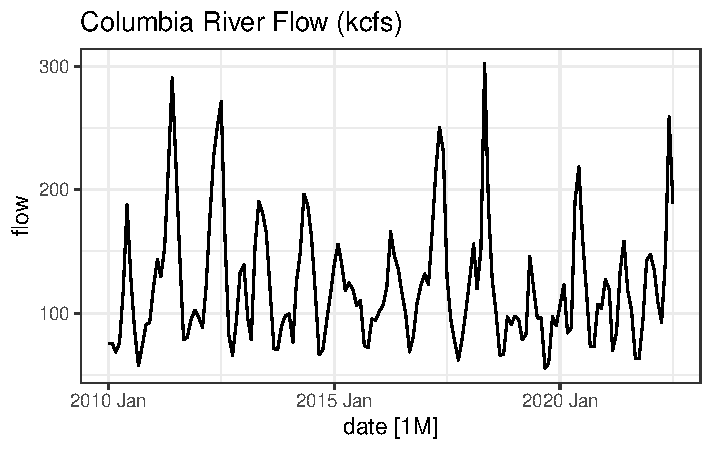
\includegraphics{Paper_files/figure-pdf/unnamed-chunk-1-1.pdf}

}

\end{figure}

\hypertarget{methods}{%
\subsubsection{Methods}\label{methods}}

\hypertarget{section-1}{%
\paragraph{}\label{section-1}}

\begin{Shaded}
\begin{Highlighting}[]
\NormalTok{train }\SpecialCharTok{\%\textgreater{}\%} 
  \FunctionTok{gg\_season}\NormalTok{(flow) }\SpecialCharTok{+}
  \FunctionTok{ggtitle}\NormalTok{(}\StringTok{"Seasonality Plot: Columbia River Flow (kcfs)"}\NormalTok{) }\SpecialCharTok{+}
  \FunctionTok{xlab}\NormalTok{(}\StringTok{"Month"}\NormalTok{) }\SpecialCharTok{+}
  \FunctionTok{theme}\NormalTok{(}\AttributeTok{legend.position =} \FunctionTok{c}\NormalTok{(.}\DecValTok{9}\NormalTok{, .}\DecValTok{7}\NormalTok{))}
\end{Highlighting}
\end{Shaded}

\begin{figure}[H]

{\centering 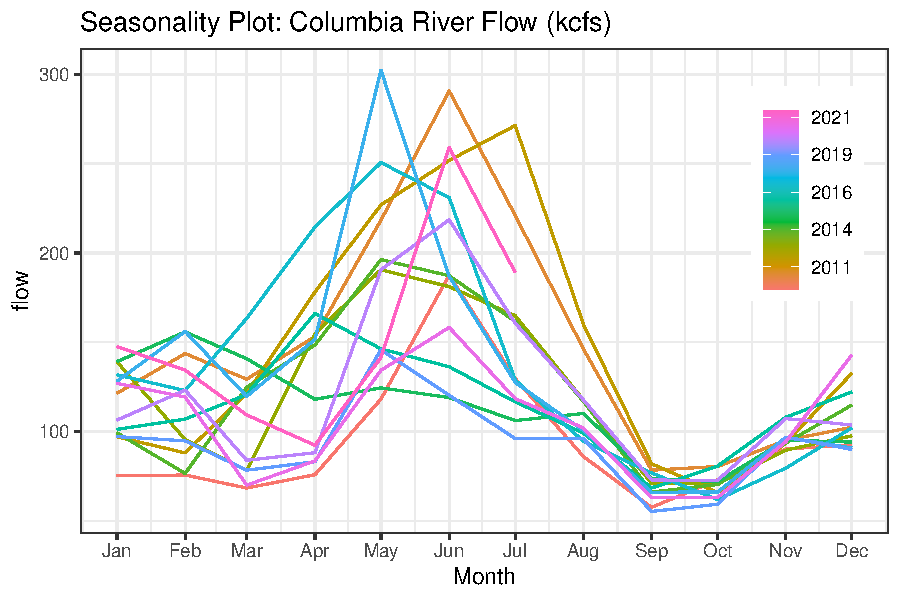
\includegraphics{Paper_files/figure-pdf/unnamed-chunk-2-1.pdf}

}

\end{figure}

\hypertarget{linear-model}{%
\subparagraph{\texorpdfstring{\textbf{Linear
Model}}{Linear Model}}\label{linear-model}}

The linear model is a tried and true model used in various situations.
For flow prediction, only the seasonality, or month, will be used as an
exogenous factor. While climate change may introduce a trend to river
flows in the very long run, a trend will not be included in this model
since we are not making long-term predictions. As such, this model will
predict the monthly average within the training set for each month in
the test set.

\hypertarget{ets}{%
\subparagraph{\texorpdfstring{\textbf{ETS}}{ETS}}\label{ets}}

The ETS model will be estimated for the level and seasonality. Once
again, and for similar reasons, a trend will not be included.

\hypertarget{arima}{%
\subparagraph{\texorpdfstring{\textbf{ARIMA}}{ARIMA}}\label{arima}}

The ARIMA model will be determined through the Hyndman-Khandakar
algorithm as specified in the \emph{fable} package.

\begin{Shaded}
\begin{Highlighting}[]
\NormalTok{train }\SpecialCharTok{\%\textgreater{}\%} 
  \FunctionTok{gg\_tsdisplay}\NormalTok{(}
    \CommentTok{\#difference(flow, 12) \%\textgreater{}\% difference(),}
\NormalTok{    flow,}
    \AttributeTok{plot\_type =} \StringTok{"partial"}\NormalTok{, }\AttributeTok{lag\_max =} \DecValTok{36}
\NormalTok{  )}
\end{Highlighting}
\end{Shaded}

\begin{figure}[H]

{\centering 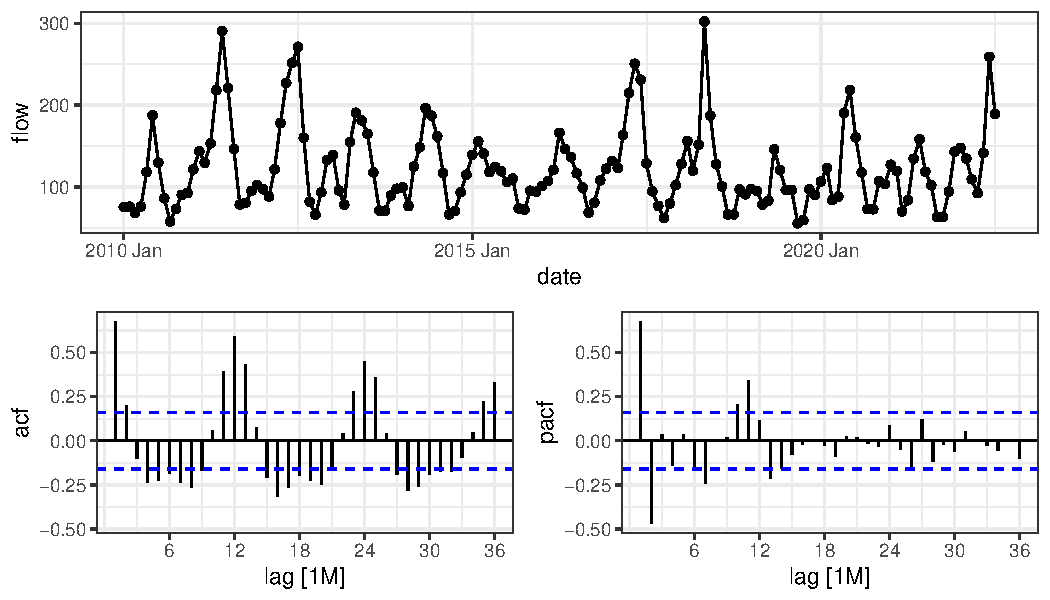
\includegraphics{Paper_files/figure-pdf/unnamed-chunk-3-1.pdf}

}

\end{figure}

\hypertarget{results}{%
\subsubsection{Results}\label{results}}

The estimated models produced the following forecasts on the test set:

\hypertarget{section-2}{%
\paragraph{}\label{section-2}}

\begin{Shaded}
\begin{Highlighting}[]
\NormalTok{fx }\SpecialCharTok{\%\textgreater{}\%} 
  \FunctionTok{autoplot}\NormalTok{(}
\NormalTok{    data }\SpecialCharTok{\%\textgreater{}\%} \FunctionTok{filter}\NormalTok{(}\FunctionTok{year}\NormalTok{(date)}\SpecialCharTok{\textgreater{}}\DecValTok{2021}\NormalTok{),}
    \CommentTok{\# level = NULL}
\NormalTok{  ) }\SpecialCharTok{+}
  \FunctionTok{ggtitle}\NormalTok{(}\StringTok{"Monthly Columbia River Flow Out{-}of{-}Sample Forecasts"}\NormalTok{) }\SpecialCharTok{+}
  \FunctionTok{facet\_grid}\NormalTok{(.model }\SpecialCharTok{\textasciitilde{}}\NormalTok{ .) }\SpecialCharTok{+}
  \FunctionTok{geom\_label}\NormalTok{(}
    \AttributeTok{data =}\NormalTok{ fx }\SpecialCharTok{\%\textgreater{}\%} 
      \FunctionTok{accuracy}\NormalTok{(}
\NormalTok{        test, }
        \AttributeTok{measures =} \FunctionTok{list}\NormalTok{(point\_accuracy\_measures, distribution\_accuracy\_measures)}
\NormalTok{      ),}
    \FunctionTok{aes}\NormalTok{(}\AttributeTok{x =} \SpecialCharTok{{-}}\ConstantTok{Inf}\NormalTok{, }\AttributeTok{y =} \ConstantTok{Inf}\NormalTok{, }\AttributeTok{label =} \FunctionTok{paste}\NormalTok{(}
      \StringTok{" RMSE:"}\NormalTok{, }\FunctionTok{round}\NormalTok{(RMSE, }\DecValTok{1}\NormalTok{),}
      \StringTok{"}\SpecialCharTok{\textbackslash{}n}\StringTok{"}\NormalTok{, }\StringTok{"MAPE: "}\NormalTok{, }\FunctionTok{round}\NormalTok{(MAPE, }\DecValTok{1}\NormalTok{),}
      \StringTok{"}\SpecialCharTok{\textbackslash{}n}\StringTok{"}\NormalTok{, }\StringTok{"CRPS: "}\NormalTok{, }\FunctionTok{round}\NormalTok{(CRPS, }\DecValTok{1}\NormalTok{)}
\NormalTok{    )),}
    \AttributeTok{hjust =} \DecValTok{0}\NormalTok{, }\AttributeTok{vjust =} \DecValTok{1}
\NormalTok{  )}
\end{Highlighting}
\end{Shaded}

\begin{figure}[H]

{\centering 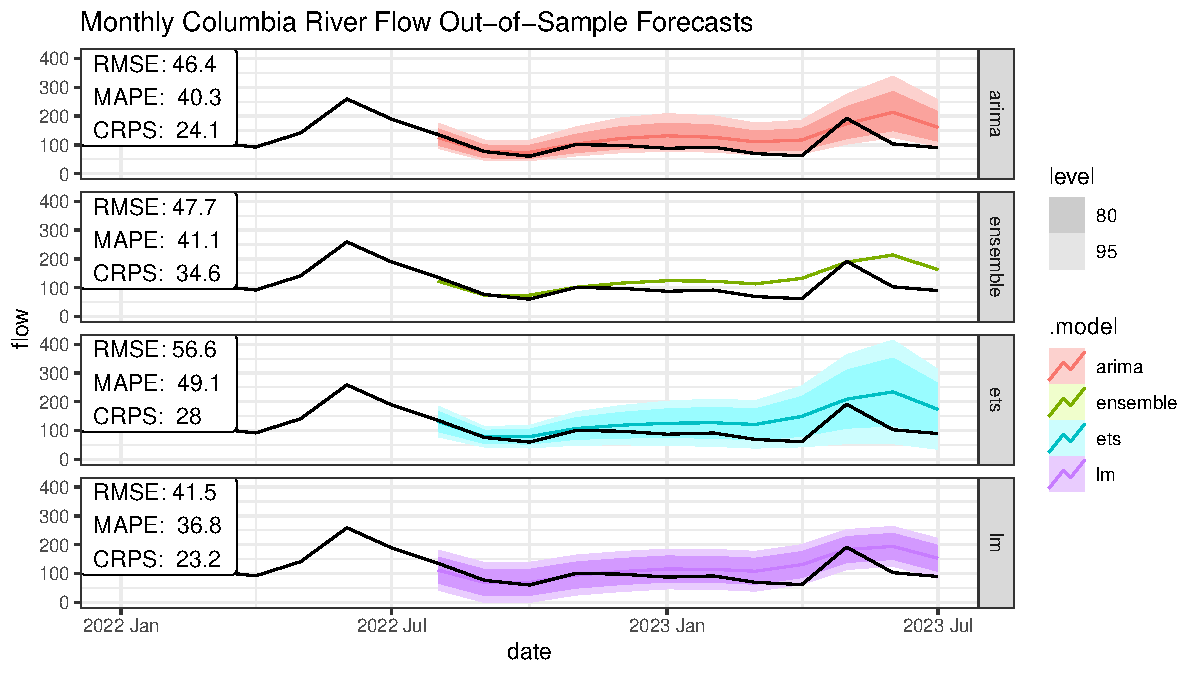
\includegraphics{Paper_files/figure-pdf/unnamed-chunk-4-1.pdf}

}

\end{figure}

ARIMA Statistics:

\begin{Shaded}
\begin{Highlighting}[]
\NormalTok{fit }\SpecialCharTok{\%\textgreater{}\%} 
  \FunctionTok{select}\NormalTok{(arima) }\SpecialCharTok{\%\textgreater{}\%} 
  \FunctionTok{report}\NormalTok{()}
\end{Highlighting}
\end{Shaded}

\begin{verbatim}
Series: flow 
Model: ARIMA(1,0,2)(0,1,2)[12] 
Transformation: log(flow) 

Coefficients:
        ar1     ma1      ma2     sma1     sma2
      0.747  0.1019  -0.2630  -0.6553  -0.1901
s.e.  0.146  0.1765   0.1429   0.1324   0.1102

sigma^2 estimated as 0.03121:  log likelihood=39.23
AIC=-66.46   AICc=-65.82   BIC=-48.85
\end{verbatim}

ETS Statistics:

\begin{Shaded}
\begin{Highlighting}[]
\NormalTok{fit }\SpecialCharTok{\%\textgreater{}\%} 
  \FunctionTok{select}\NormalTok{(ets) }\SpecialCharTok{\%\textgreater{}\%} 
  \FunctionTok{report}\NormalTok{()}
\end{Highlighting}
\end{Shaded}

\begin{verbatim}
Series: flow 
Model: ETS(M,N,M) 
  Smoothing parameters:
    alpha = 0.4867502 
    gamma = 0.0001012484 

  Initial states:
     l[0]      s[0]     s[-1]     s[-2]     s[-3]     s[-4]    s[-5]    s[-6]
 123.8028 0.8609289 0.7784877 0.5741357 0.5696651 0.9538401 1.258872 1.695363
    s[-7]    s[-8]     s[-9]    s[-10]   s[-11]
 1.512702 1.081726 0.8805814 0.9235965 0.910102

  sigma^2:  0.0425

     AIC     AICc      BIC 
1728.484 1732.040 1773.743 
\end{verbatim}

\hypertarget{section-3}{%
\paragraph{}\label{section-3}}

\hypertarget{discussion}{%
\subsubsection{Discussion}\label{discussion}}

The LM does minimize the RMSE, MAPE, and CRPS. A complicating factor is
that while strong seasonality does exist, the amount of water in a given
year varies by a good margin as do the springs. A cold spring that
suddenly turns hot will cause snow to melt faster causing large peaks.
In contrast, a warm spring will cause the snow to begin melting earlier,
but not necessarily at a fast rate. The linear model predicts each month
to be the historical average, producing a decent forecast.

The ETS and ARIMA models both overestimate the actual flow, likely a
result of the high water year for the last period of the training set.
The positive ma1 term and negative ma2 term indicate that when there is
this large change in the flow, the following month is usually the same
direction, but the month after that results in a larger contraction in
the opposite direction. This lines up with the warm/cold spring theory
postulated in the previous paragraph.

A gamma value near zero in the ETS model indicates that river flows do
not respond very much to changes in the prior season. The alpha equal to
almost .5 indicates some response to recent months, but not overly so.
Together these help explain why the linear model outperformed the other
two, more complicated models: the prior years' values are not a good
indicator for the current year, and recent months can only go so far.
When no exogenous variables are considered, this is nearly a random
walk, for which the historical mean is the best approximate.

\hypertarget{conclusion}{%
\subsubsection{Conclusion}\label{conclusion}}

Medium and long term predictions of river flows are very difficult
without exogenous factors. The higher correlation with more recent
periods could imply that short-term forecasts are more achievable. A
good approach for the long term is to simply use the historical average,
an ARIMA model may prove useful for the shorter term forecasts. Further
study using cross validation should be done to determine if a modified
ensemble method could be beneficial where the ARIMA model is given a
higher weight for the first couple of months and the linear model
thereafter.



\end{document}
